\chapter{Derivation of \texorpdfstring{$\Phi$}{Φ}} \label{sec:analytical-energy}
    \todoitemone{$R$ used here, $r$ used elsewhere}
    
    Here, we outline the derivation of $\Phi$, which is used in \S\ref{sec:nutrient-uptake:variation-of-vessels} as the approximation
    \begin{equation*}
        \Phi(N_\text{A}, N_\text{V}) \approx \frac{E_\text{kinetic}(\Gamma_\text{in}) - E_\text{kinetic}(\Gamma_\text{out})}{E_\text{kinetic}(\Gamma_\text{in})}.
    \end{equation*}

    We begin by considering Figure \ref{fig:analytical-expression-placenta}, which shows a simplified view of the inlets and outlets in the placenta, which has $N_\text{A}$ arteries, $N_\text{V}$ basal plate and septal wall veins, and $2$ marginal sinus veins; this reflects the problem setup throughout \S\ref{sec:nutrient-uptake:variation-of-vessels}. The flux of blood, $Q$, through each inlet and outlet is calculated as
    \begin{equation}
        Q = \frac{4 U R}{3},
    \end{equation}
    where we have assumed a Poiseuille flow of peak $U$ and radius $R$. The peak inflow speeds for the arteries are given as $\{ U_{\text{in},1}, ..., U_{\text{in},N_\text{A}} \}$ with artery radius $R_\text{a}$, therefore giving fluxes $$Q_\text{in} := \{ U_{\text{in},j} R_\text{A} \}_j.$$ Similarly, fluxes through the basal plate and septal wall veins are given as $$Q_\text{out} := \{ U_{\text{out},j} R_\text{V} \}_j,$$ and fluxes through marginal sinus veins are given as $$\{ Q^\text{ms}_\text{out} := U^\text{ms}_{\text{out},1} R^\text{ms}_\text{V}, U^\text{ms}_{\text{out},2} R^\text{ms}_\text{V} \}.$$
    
    \begin{figure}
        \centering
        

\tikzset{every picture/.style={line width=0.75pt}} %set default line width to 0.75pt        

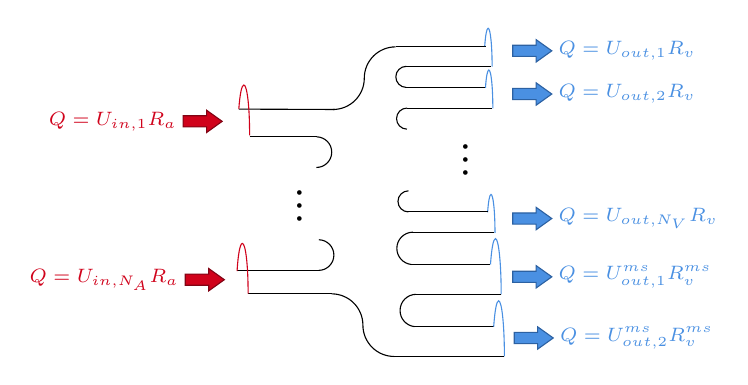
\begin{tikzpicture}[x=0.75pt,y=0.75pt,yscale=-1,xscale=1]
%uncomment if require: \path (0,300); %set diagram left start at 0, and has height of 300

%Straight Lines [id:da6897475479741801] 
\draw    (182.17,71.91) -- (228.6,72.09) ;
%Straight Lines [id:da9207632072413952] 
\draw    (187.34,85.27) -- (219.69,85.27) ;
%Shape: Arc [id:dp5144902494751977] 
\draw  [draw opacity=0] (242.63,57) .. controls (242.63,65.33) and (235.88,72.09) .. (227.56,72.09) -- (227.55,57.01) -- cycle ; \draw   (242.63,57) .. controls (242.63,65.33) and (235.88,72.09) .. (227.56,72.09) ;  
%Shape: Arc [id:dp044092686186237184] 
\draw  [draw opacity=0] (242.63,57) .. controls (242.63,48.67) and (249.38,41.92) .. (257.71,41.92) -- (257.71,57) -- cycle ; \draw   (242.63,57) .. controls (242.63,48.67) and (249.38,41.92) .. (257.71,41.92) ;  
%Straight Lines [id:da7127120437770351] 
\draw    (257.71,41.92) -- (301.07,41.92) ;
%Straight Lines [id:da36592894326131375] 
\draw    (262.91,51.29) -- (303.82,51.29) ;
%Shape: Arc [id:dp8073218791002419] 
\draw  [draw opacity=0] (262.82,61.46) .. controls (260.05,61.41) and (257.82,59.15) .. (257.82,56.37) .. controls (257.82,53.56) and (260.1,51.29) .. (262.91,51.29) -- (262.91,56.37) -- cycle ; \draw   (262.82,61.46) .. controls (260.05,61.41) and (257.82,59.15) .. (257.82,56.37) .. controls (257.82,53.56) and (260.1,51.29) .. (262.91,51.29) ;  
%Shape: Arc [id:dp9115427482667546] 
\draw  [draw opacity=0] (257.04,191.08) .. controls (248.71,191.08) and (241.96,184.32) .. (241.96,175.99) -- (257.04,175.99) -- cycle ; \draw   (257.04,191.08) .. controls (248.71,191.08) and (241.96,184.32) .. (241.96,175.99) ;  
%Shape: Arc [id:dp40739579709299334] 
\draw  [draw opacity=0] (226.88,160.91) .. controls (235.2,160.91) and (241.96,167.67) .. (241.96,175.99) -- (226.88,175.99) -- cycle ; \draw   (226.88,160.91) .. controls (235.2,160.91) and (241.96,167.67) .. (241.96,175.99) ;  
%Straight Lines [id:da315564227105416] 
\draw    (186.63,160.91) -- (226.88,160.91) ;
%Shape: Arc [id:dp06802366651187608] 
\draw  [draw opacity=0] (220.73,134.85) .. controls (224.75,134.92) and (227.98,138.2) .. (227.98,142.23) .. controls (227.98,146.3) and (224.68,149.61) .. (220.61,149.61) -- (220.61,142.23) -- cycle ; \draw   (220.73,134.85) .. controls (224.75,134.92) and (227.98,138.2) .. (227.98,142.23) .. controls (227.98,146.3) and (224.68,149.61) .. (220.61,149.61) ;  
%Straight Lines [id:da27217516789748486] 
\draw    (181.45,149.61) -- (220.61,149.61) ;
%Shape: Arc [id:dp1353432404024142] 
\draw  [draw opacity=0] (219.69,85.27) .. controls (223.71,85.33) and (226.94,88.61) .. (226.94,92.64) .. controls (226.94,96.72) and (223.64,100.02) .. (219.57,100.02) -- (219.57,92.64) -- cycle ; \draw   (219.69,85.27) .. controls (223.71,85.33) and (226.94,88.61) .. (226.94,92.64) .. controls (226.94,96.72) and (223.64,100.02) .. (219.57,100.02) ;  
%Shape: Arc [id:dp238698053685636] 
\draw  [draw opacity=0] (182.17,71.91) .. controls (182.66,64.96) and (183.56,60.28) .. (184.6,60.28) .. controls (186.13,60.28) and (187.37,70.68) .. (187.36,83.51) .. controls (187.36,83.85) and (187.35,84.19) .. (187.35,84.52) -- (184.57,83.51) -- cycle ; \draw  [color={rgb, 255:red, 208; green, 2; blue, 27 }  ,draw opacity=1 ] (182.17,71.91) .. controls (182.66,64.96) and (183.56,60.28) .. (184.6,60.28) .. controls (186.13,60.28) and (187.37,70.68) .. (187.36,83.51) .. controls (187.36,83.85) and (187.35,84.19) .. (187.35,84.52) ;  
%Shape: Arc [id:dp8213186661755791] 
\draw  [draw opacity=0] (181.34,150.01) .. controls (181.79,142.1) and (182.76,136.62) .. (183.87,136.62) .. controls (185.41,136.62) and (186.65,147.02) .. (186.64,159.85) .. controls (186.63,160.19) and (186.63,160.53) .. (186.63,160.86) -- (183.85,159.85) -- cycle ; \draw  [color={rgb, 255:red, 208; green, 2; blue, 27 }  ,draw opacity=1 ] (181.34,150.01) .. controls (181.79,142.1) and (182.76,136.62) .. (183.87,136.62) .. controls (185.41,136.62) and (186.65,147.02) .. (186.64,159.85) .. controls (186.63,160.19) and (186.63,160.53) .. (186.63,160.86) ;  
%Shape: Arc [id:dp20383419320801943] 
\draw  [draw opacity=0] (300.66,41.52) .. controls (301.01,36.36) and (301.61,32.94) .. (302.3,32.94) .. controls (303.36,32.94) and (304.22,41.22) .. (304.21,51.44) -- (302.28,51.47) -- cycle ; \draw  [color={rgb, 255:red, 74; green, 144; blue, 226 }  ,draw opacity=1 ] (300.66,41.52) .. controls (301.01,36.36) and (301.61,32.94) .. (302.3,32.94) .. controls (303.36,32.94) and (304.22,41.22) .. (304.21,51.44) ;  
%Straight Lines [id:da9273006738288603] 
\draw    (263.26,71.4) -- (304.17,71.4) ;
%Shape: Arc [id:dp20008369967725814] 
\draw  [draw opacity=0] (263.17,81.57) .. controls (260.4,81.52) and (258.17,79.26) .. (258.17,76.48) .. controls (258.17,73.67) and (260.45,71.4) .. (263.26,71.4) -- (263.26,76.48) -- cycle ; \draw   (263.17,81.57) .. controls (260.4,81.52) and (258.17,79.26) .. (258.17,76.48) .. controls (258.17,73.67) and (260.45,71.4) .. (263.26,71.4) ;  
%Shape: Arc [id:dp8626799595145647] 
\draw  [draw opacity=0] (301.01,61.63) .. controls (301.35,56.47) and (301.96,53.05) .. (302.64,53.05) .. controls (303.71,53.05) and (304.56,61.33) .. (304.56,71.55) -- (302.63,71.58) -- cycle ; \draw  [color={rgb, 255:red, 74; green, 144; blue, 226 }  ,draw opacity=1 ] (301.01,61.63) .. controls (301.35,56.47) and (301.96,53.05) .. (302.64,53.05) .. controls (303.71,53.05) and (304.56,61.33) .. (304.56,71.55) ;  
%Straight Lines [id:da0589129492536995] 
\draw    (262.82,61.46) -- (301.01,61.46) ;
%Straight Lines [id:da30421383578476013] 
\draw    (264.3,131.38) -- (305.21,131.38) ;
%Shape: Arc [id:dp200178610381043] 
\draw  [draw opacity=0] (265.25,146.76) .. controls (261.35,146.33) and (258.31,143.02) .. (258.31,139) .. controls (258.31,134.69) and (261.8,131.2) .. (266.11,131.2) -- (266.11,139) -- cycle ; \draw   (265.25,146.76) .. controls (261.35,146.33) and (258.31,143.02) .. (258.31,139) .. controls (258.31,134.69) and (261.8,131.2) .. (266.11,131.2) ;  
%Shape: Arc [id:dp4498403889935414] 
\draw  [draw opacity=0] (302.05,121.62) .. controls (302.39,116.46) and (303,113.04) .. (303.68,113.04) .. controls (304.75,113.04) and (305.6,121.32) .. (305.6,131.54) -- (303.67,131.57) -- cycle ; \draw  [color={rgb, 255:red, 74; green, 144; blue, 226 }  ,draw opacity=1 ] (302.05,121.62) .. controls (302.39,116.46) and (303,113.04) .. (303.68,113.04) .. controls (304.75,113.04) and (305.6,121.32) .. (305.6,131.54) ;  
%Straight Lines [id:da22468899311040502] 
\draw    (263.86,121.44) -- (302.05,121.44) ;
%Shape: Arc [id:dp19536738802800802] 
\draw  [draw opacity=0] (263.86,121.44) .. controls (261.09,121.4) and (258.86,119.14) .. (258.86,116.36) .. controls (258.86,113.55) and (261.14,111.27) .. (263.95,111.27) -- (263.95,116.36) -- cycle ; \draw   (263.86,121.44) .. controls (261.09,121.4) and (258.86,119.14) .. (258.86,116.36) .. controls (258.86,113.55) and (261.14,111.27) .. (263.95,111.27) ;  
%Straight Lines [id:da522381672409731] 
\draw    (265.25,146.76) -- (303.43,146.76) ;
%Shape: Arc [id:dp7499727362361837] 
\draw  [draw opacity=0] (303.43,146.76) .. controls (303.94,139.28) and (304.81,134.32) .. (305.81,134.32) .. controls (307.35,134.32) and (308.59,146.32) .. (308.58,161.14) -- (305.78,161.19) -- cycle ; \draw  [color={rgb, 255:red, 74; green, 144; blue, 226 }  ,draw opacity=1 ] (303.43,146.76) .. controls (303.94,139.28) and (304.81,134.32) .. (305.81,134.32) .. controls (307.35,134.32) and (308.59,146.32) .. (308.58,161.14) ;  
%Straight Lines [id:da4989617610080148] 
\draw    (267.66,161.14) -- (308.58,161.14) ;
%Shape: Arc [id:dp47436356415299286] 
\draw  [draw opacity=0] (266.8,176.69) .. controls (262.9,176.26) and (259.86,172.96) .. (259.86,168.94) .. controls (259.86,164.63) and (263.35,161.14) .. (267.66,161.14) -- (267.66,168.94) -- cycle ; \draw   (266.8,176.69) .. controls (262.9,176.26) and (259.86,172.96) .. (259.86,168.94) .. controls (259.86,164.63) and (263.35,161.14) .. (267.66,161.14) ;  
%Straight Lines [id:da47731005062437015] 
\draw    (266.8,176.69) -- (304.98,176.69) ;
%Shape: Arc [id:dp6764201761859778] 
\draw  [draw opacity=0] (304.98,176.69) .. controls (305.49,169.22) and (306.36,164.26) .. (307.35,164.26) .. controls (308.9,164.26) and (310.14,176.26) .. (310.13,191.08) -- (307.33,191.13) -- cycle ; \draw  [color={rgb, 255:red, 74; green, 144; blue, 226 }  ,draw opacity=1 ] (304.98,176.69) .. controls (305.49,169.22) and (306.36,164.26) .. (307.35,164.26) .. controls (308.9,164.26) and (310.14,176.26) .. (310.13,191.08) ;  
%Straight Lines [id:da8107752914505761] 
\draw    (257.04,191.08) -- (310.13,191.08) ;
%Right Arrow [id:dp2469458095146153] 
\draw  [color={rgb, 255:red, 129; green, 4; blue, 20 }  ,draw opacity=1 ][fill={rgb, 255:red, 208; green, 2; blue, 27 }  ,fill opacity=1 ] (155.35,75.12) -- (166.64,75.12) -- (166.64,72.44) -- (174.16,77.81) -- (166.64,83.19) -- (166.64,80.5) -- (155.35,80.5) -- cycle ;
%Right Arrow [id:dp9958402750896171] 
\draw  [color={rgb, 255:red, 44; green, 97; blue, 162 }  ,draw opacity=1 ][fill={rgb, 255:red, 74; green, 144; blue, 226 }  ,fill opacity=1 ] (314.16,41.14) -- (325.45,41.14) -- (325.45,38.46) -- (332.97,43.83) -- (325.45,49.21) -- (325.45,46.52) -- (314.16,46.52) -- cycle ;
%Right Arrow [id:dp6128543836231557] 
\draw  [color={rgb, 255:red, 44; green, 97; blue, 162 }  ,draw opacity=1 ][fill={rgb, 255:red, 74; green, 144; blue, 226 }  ,fill opacity=1 ] (314.16,61.95) -- (325.45,61.95) -- (325.45,59.26) -- (332.97,64.64) -- (325.45,70.01) -- (325.45,67.32) -- (314.16,67.32) -- cycle ;
%Right Arrow [id:dp7930204983840552] 
\draw  [color={rgb, 255:red, 44; green, 97; blue, 162 }  ,draw opacity=1 ][fill={rgb, 255:red, 74; green, 144; blue, 226 }  ,fill opacity=1 ] (314.16,121.94) -- (325.45,121.94) -- (325.45,119.25) -- (332.97,124.62) -- (325.45,130) -- (325.45,127.31) -- (314.16,127.31) -- cycle ;
%Right Arrow [id:dp8020822248149451] 
\draw  [color={rgb, 255:red, 44; green, 97; blue, 162 }  ,draw opacity=1 ][fill={rgb, 255:red, 74; green, 144; blue, 226 }  ,fill opacity=1 ] (314.16,150.02) -- (325.45,150.02) -- (325.45,147.33) -- (332.97,152.71) -- (325.45,158.08) -- (325.45,155.4) -- (314.16,155.4) -- cycle ;
%Right Arrow [id:dp05601739812042572] 
\draw  [color={rgb, 255:red, 44; green, 97; blue, 162 }  ,draw opacity=1 ][fill={rgb, 255:red, 74; green, 144; blue, 226 }  ,fill opacity=1 ] (314.86,179.49) -- (326.14,179.49) -- (326.14,176.81) -- (333.67,182.18) -- (326.14,187.56) -- (326.14,184.87) -- (314.86,184.87) -- cycle ;
%Right Arrow [id:dp45340586186745924] 
\draw  [color={rgb, 255:red, 129; green, 4; blue, 20 }  ,draw opacity=1 ][fill={rgb, 255:red, 208; green, 2; blue, 27 }  ,fill opacity=1 ] (156.39,151.41) -- (167.68,151.41) -- (167.68,148.72) -- (175.21,154.1) -- (167.68,159.47) -- (167.68,156.78) -- (156.39,156.78) -- cycle ;

% Text Node
\draw (291.46,96.24) node  [font=\LARGE,rotate=-90]  {$...$};
% Text Node
\draw (211.77,118.4) node  [font=\LARGE,rotate=-90]  {$...$};
% Text Node
\draw (153.35,77.81) node [anchor=east] [inner sep=0.75pt]  [font=\scriptsize,color={rgb, 255:red, 208; green, 2; blue, 27 }  ,opacity=1 ]  {$Q=U_{\text{in} ,1} R_{\text{a}}$};
% Text Node
\draw (154.39,154.1) node [anchor=east] [inner sep=0.75pt]  [font=\scriptsize,color={rgb, 255:red, 208; green, 2; blue, 27 }  ,opacity=1 ]  {$Q=U_{\text{in} ,N_{\text{A}}} R_{\text{a}}$};
% Text Node
\draw (334.97,43.83) node [anchor=west] [inner sep=0.75pt]  [font=\scriptsize,color={rgb, 255:red, 74; green, 144; blue, 226 }  ,opacity=1 ]  {$Q=U_{out,1} R_{\text{v}}$};
% Text Node
\draw (334.97,64.64) node [anchor=west] [inner sep=0.75pt]  [font=\scriptsize,color={rgb, 255:red, 74; green, 144; blue, 226 }  ,opacity=1 ]  {$Q=U_{out,2} R_{\text{v}}$};
% Text Node
\draw (334.97,124.62) node [anchor=west] [inner sep=0.75pt]  [font=\scriptsize,color={rgb, 255:red, 74; green, 144; blue, 226 }  ,opacity=1 ]  {$Q=U_{out,N_{\text{V}}} R_{\text{v}}$};
% Text Node
\draw (334.97,152.71) node [anchor=west] [inner sep=0.75pt]  [font=\scriptsize,color={rgb, 255:red, 74; green, 144; blue, 226 }  ,opacity=1 ]  {$Q=U_{out,1}^{\text{ms}} R_{\text{v}}^{\text{ms}}$};
% Text Node
\draw (335.67,182.18) node [anchor=west] [inner sep=0.75pt]  [font=\scriptsize,color={rgb, 255:red, 74; green, 144; blue, 226 }  ,opacity=1 ]  {$Q=U_{out,2}^{\text{ms}} R_{\text{v}}^{\text{ms}}$};


\end{tikzpicture}

        \caption{Caption}
        \label{fig:analytical-expression-placenta}
    \end{figure}

    Assuming conservation of mass (i.e. the flux in equals the flux out), we get
    \begin{equation}
        \sum_{j=1}^{N_\text{A}} \frac{4 U_{\text{in},j} R_\text{a}}{3} = \sum_{j=1}^{N_\text{v}} \frac{4 U_{\text{out},j} R_\text{v}}{3} + \sum_{j=1}^{2} \frac{4 U^\text{ms}_{\text{out},j} R^\text{ms}_\text{v}}{3}.
        \label{eq:analytical-expression-conservation-of-mass}
    \end{equation}

    We recall the vessel sizes from Table \ref{tab:structural-parameters} that $R_\text{A} = \qty{0.5}{\milli\metre}$, $R_\text{V} = \qty{1.5}{\milli\metre}$, and $R^\text{ms}_\text{V} = \qty{3}{\milli\metre}$. This means we have the relation $R^\text{ms}_\text{V} = 2R_\text{V} = 6R_\text{A}$.

    Next, we make an assumption of equal flow peaks on each similar vessel; this involves taking
    \begin{alignat*}{5}
        U_\text{in} & := U_{\text{in},i} && = U_{\text{in},j} && \text{ for } i \neq j, \\
        U_\text{out} & := U_{\text{out},i} && = U_{\text{out},j} && \text{ for } i \neq j, \\
        U^\text{ms}_\text{out} & := U^\text{ms}_{\text{out},1} && = U^\text{ms}_{\text{out},2}. &&
    \end{alignat*}
    We also make the assumption that peak outflow speeds are fractions of the inflow peak speed:
    \begin{align*}
        U_\text{out} & = k_1 U_\text{in}, \\
        U^\text{ms}_\text{out} & = k_2 U_\text{in}, \\
    \end{align*}
    where $k_1$ and $k_2$ are constants. These assumptions allow us to rearrange Equation \eqref{eq:analytical-expression-conservation-of-mass} to give
    \begin{equation}
        k_2 = \frac{N_\text{A}-3N_\text{V}k_1}{12}.
        \label{eq:k2-1}
    \end{equation}

    We make the assumption that fluxes out of an individual basal plate or septal wall vein is equal to twice the flux out of a marginal sinus vein, which accounts for the fact that basal plate and septal wall veins are preferable due to their proximity to arteries. We therefore set. $U_\text{out}R_\text{V} = 2U^\text{ms}_\text{out}R^\text{ms}_\text{V}$ and then obtain
    \begin{equation}
        k_2 = \frac{k_1}{4}.
        \label{eq:k2-2}
    \end{equation}
    Using Equations \eqref{eq:k2-1} and \eqref{eq:k2-2} to solve for $k_1$, we get
    \begin{equation}
        k_1 = \frac{N_\text{A}}{3(2 + N_\text{V})}.
    \end{equation}

    Next, the kinetic energy on all inlets and outlets is respectively given by
    \begin{align*}
        E_\text{kinetic}(\Gamma_\text{in}) & = \frac{N_\text{A}}{2} \int_{\Gamma_\text{in}} |U_\text{in}|^2 \diff s, \\
        E_\text{kinetic}(\Gamma_\text{in}) & = \frac{N_\text{V}}{2} \int_{\Gamma_\text{out}} |U_\text{out}|^2 \diff s + \frac{2}{2} \int_{\Gamma^\text{ms}_\text{out}} |U^\text{ms}_\text{out}|^2 \diff s.
    \end{align*}
    Simplifying these expressions with our previous assumptions gives
    \begin{align}
        E_\text{kinetic}(\Gamma_\text{in}) & = \frac{8 N_\text{A} U_\text{in}^2 R_\text{A}}{15}, \\
        E_\text{kinetic}(\Gamma_\text{out}) & = \frac{8 N_\text{V} U_\text{out}^2 R_\text{V}}{15} + \frac{16 (U^\text{ms}_\text{out})^2 R^\text{ms}_\text{V}}{15}.
    \end{align}
    Taking the kinetic energy flux loss ratio as described in \S\ref{sec:nutrient-uptake:variation-of-vessels}, we arrive our approximate expression:
    \begin{equation}
        \Phi(N_\text{A}, N_\text{V}) := \frac{N_\text{A} - 3N_\text{V}k_1^2 - 12k_2^2}{N_\text{A}}.
    \end{equation}